\section{Лекция 5 (6.10)}

\subsection{Оптимальные значения параметров алгоритма SIMPLE}

Введем обозначение
\begin{equation*}
\label{eq:ns2d-simple-e}
E = \frac{4\tau}{\Ren\,{\rm H}(h_x^2, h_y^2)}
\end{equation*}
где ${\rm H}(a, b)$ -- среднее гармоническое, определяемое как
$$
{\rm H}(a, b) = \frac{2\,a\,b}{a+b}.
$$
Значение $E$ -- есть диагональное компонента матрицы диффузии
в аппроксимированных уравнениях движения (второе слагаемое в правой части первой формулы \cref{eq:ns2d_au}).

При независимом задании релаксаций по скорости и давлению,
оптимальной сходимости соответствуют значения
\begin{align*}
&E = 1 \hence \tau = \frac{\Ren \,{\rm H}(h_x^2, h_y^2)}{4}, \\
&\alpha_p = 0.8.
\end{align*}
Ещё более эффективной сходимости соответствуют параметры
\begin{equation}
\label{eq:ns2d-simplec}
E \approx 4, \quad \alpha_p = \frac{1}{1+E}.
\end{equation}
Это выражение соответствует алгоритму SIMPLEC (согласованный алгоритм, SIMPLE Consistent).

\subsection{Нестационарное уравнение Навье-Стокса}
\label{sec:ns2d-nonstat}

Запишем безразмерную систему \eqref{eq:ns2d_u} -- \eqref{eq:ns2d_div} в нестационарной постановке
\begin{equation}
\label{eq:ns2d_nonstat}
\begin{array}{l}
    \ddfr{u}{t} + \ddfr{u^2}{x} + \ddfr{uv}{y} =
        -\ddfr{p}{x}
        + \dfrac{1}{\Ren}\left(\ddfrq{u}{x} + \ddfrq{u}{y}\right),\\[10pt]
    \ddfr{v}{t} + \ddfr{uv}{x} + \ddfr{v^2}{y} =
        -\ddfr{p}{y}
        + \dfrac{1}{\Ren}\left(\ddfrq{v}{x} + \ddfrq{v}{y}\right), \\[10pt]
    \ddfr{u}{x} + \ddfr{v}{y} = 0.
\end{array}
\end{equation}
Характерное время, на которое было произведено обезразмериваение,
равно $t^0 = L/U$.

\subsubsection{Cхема расчёта по алгоритму SIMPLE}
\label{sec:simple-nonstat-algo}

Производную по времени будет аппроксимировать по двухслойной неявной схеме.
\begin{equation*}
\dfr{u}{t} = \frac{\hat u - \check u}{\dt} + o(\dt),
\end{equation*}
где символом $\check\cdot$ обозначены значения с предыдущего временн\'{о}го слоя.

Внутри каждого временн\'{о}го слоя будем исполнять
итерационный процесс по типу \eqref{eq:ns2d_semi_u} -- \eqref{eq:ns2d_semi_div}
с добавлением дискретизованной производной по времени:

\begin{equation}
    \label{eq:ns2d_nonstat_semi}
    \begin{array}{l}
    \displaystyle
    \frac{\hat u - \check u}{\dt} + \frac{\hat u - u}{\tau} + \dfr{u \hat u}{x} + \dfr{v \hat u}{y} =
        -\dfr{\hat p}{x}
        + \frac{1}{\Ren}\left(\dfrq{\hat u}{x} + \dfrq{\hat u}{y}\right), \\[10pt]
    \displaystyle
    \frac{\hat v - \check v}{\dt} + \frac{\hat v - v}{\tau} + \dfr{u\hat v}{x} + \dfr{v \hat v}{y} =
        -\dfr{\hat p}{y}
        + \frac{1}{\Ren}\left(\dfrq{\hat v}{x} + \dfrq{\hat v}{y}\right),  \\[10pt]
    \displaystyle
    \dfr{\hat u}{x} + \dfr{\hat v}{y} = 0.
    \end{array}
\end{equation}

Далее на основе этих уравнений проведём рассуждения, аналогичные приведённым в п. \ref{sec:simple-algo}.
Уравнения для пробной скорости типа \eqref{eq:ns2d_ustar}, \eqref{eq:ns2d_vstar}
примут вид
\begin{equation}
    \label{eq:ns2d_nonstat_uvstar}
    \begin{array}{l}
    \displaystyle
    \left(1 + \frac{\tau}{\dt}\right)u^* + \tau\dfr{u u^*}{x} + \tau\dfr{v u^*}{y}
       - \frac{\tau}{\Ren}\left(\dfrq{u^*}{x} + \dfrq{u^*}{y}\right)
       = -\tau\dfr{p}{x} + u + \frac\tau\dt \check u, \\[10pt]
    \displaystyle
    \left(1 + \frac{\tau}{\dt}\right)v^* + \tau\dfr{u v^*}{x} + \tau\dfr{v v^*}{y}
       - \frac{\tau}{\Ren}\left(\dfrq{v^*}{x} + \dfrq{v^*}{y}\right)
       = -\tau\dfr{p}{y} + v + \frac\tau\dt \check v.
   \end{array}
\end{equation}

Уравнения для поправок скорости \eqref{eq:ns2d_ustroke_approx}, \eqref{eq:ns2d_vstroke_approx}
и давления \eqref{eq:ns2d_pstroke_diff}
можно оставить в неизменном виде если модифицировать входящие в них множители $d^u, d^v$.
По аналогии с \eqref{eq:ns2d_du}, \eqref{eq:ns2d_dv} запишем
\begin{equation}
    \label{eq:ns2d_nonstat_duv}
    \begin{array}{l}
    \displaystyle
    d^u = \left({\rm diag}\left(A^u\right)\right)^{-1} = 
        \left(1 + \frac\tau\dt + \frac{2\tau}{\Ren}\left(\frac{1}{h_x^2} + \frac{1}{h_y^2}\right)\right)^{-1} \\[10pt]
    \displaystyle
    d^v = \left({\rm diag}\left(A^v\right) \right)^{-1}= 
        \left(1 + \frac\tau\dt + \frac{2\tau}{\Ren}\left(\frac{1}{h_x^2} + \frac{1}{h_y^2}\right)\right)^{-1}.
    \end{array}
\end{equation}
Здесь $A^u$, $A^v$ -- матрицы левых частей выражений \eqref{eq:ns2d_nonstat_uvstar}.

Схема расчёта на временн\'{о}м слое остаётся аналогичной стационарному случаю,
с той разницей, что первая итерация использует значение расчётных полей
с предыдущего шага по времени.
Порядок действий на временном слое:

\begin{enumerate}
\item Присвоить $u=\check u$, $v=\check v$, $p=\check p$;
\item Из уравнений \eqref{eq:ns2d_nonstat_uvstar}
      вычислить значения $u^*, v^*$;
\item Определить поправку давления $p'$ из уравнения \eqref{eq:ns2d_pstroke_diff} с использованием \eqref{eq:ns2d_nonstat_duv};
\item Найти поправки скорости $u', v'$ из выражений \eqref{eq:ns2d_ustroke_approx}, \eqref{eq:ns2d_vstroke_approx} с использованием \eqref{eq:ns2d_nonstat_duv};
\item Выразить значения переменных для текущего слоя из \eqref{eq:ns2d_decomp};
      Для определения давления использовать сглаживание с коэффициентом $\alpha_p$;
\item Найти невязку с ипользованием найденных значений $\hat u, \hat v, \hat p$
      из выражения \eqref{eq:ns2d_residual}.
      Если она недостаточно мала, то выполняется присваивание
      $u = \hat u, \; v=\hat v, \; p = \hat p$ 
      и возвращение на шаг 2.
      Если сходимость достигнута, то перейти на следующий шаг по времени.
      Для этого выполнить
      $\check u = \hat u, \; \check v= \hat v, \; \check p = \hat p$ 
      и перейти на шаг 1.
\end{enumerate}


\subsection{Завихренность и функция тока}

Для несжимаемых течений ($\nabla\cdot\vec u = 0$) можно ввести векторный потенциал скорости:
\begin{equation*}
    \nabla\times\vec\Psi = \vec u
\end{equation*}

Также определим векторное поле завихренности как
\begin{equation*}
    \vec \Omega = \nabla \times \vec u
\end{equation*}

Компоненты этого вектора характеризуют вращательную составляющую скорости в
плоскостях, перпендикулярных соответствующим базисным векторам.
Например, компонента $\Omega_z$ характеризует вращение в плоскости $xy$.

Подставив векторный потенциал в выражение для завихренности, получим связь между двумя введёнными векторными полями
\begin{equation*}
    \vec \Omega = \nabla \times \left( \nabla \times \vec \Psi \right) = \nabla\left(\nabla\cdot\vec\Psi\right) - \nabla^2\vec\Psi.
\end{equation*}

Далее рассмотрим двумерные течения в декартовой системе координат. $z$-компонента
последнего выражения (с учётом $\partial/\partial z=0$) сократится до
\begin{equation*}
    \Omega_z = -\nabla^2\Psi_z
\end{equation*}
или, введя обозначения $\Omega_z = \omega$, $\Psi_z = \psi$:
\begin{align}
    \nonumber
     &\dfr{\psi}{y} = u, \\
    \label{eq:psiw_def}
    -&\dfr{\psi}{x} = v, \\
    \nonumber
     &\omega = \dfr{v}{x} - \dfr{u}{y}
\end{align}
и расписывая оператор Лапласа покоординатно
\begin{equation}
    \label{eq:psiw}
    -\left(\dfrq{\psi}{x} + \dfrq{\psi}{y}\right) = \omega.
\end{equation}

Скалярное поле $\psi$ называется функцией тока и его изолинии совпадают с линиями тока течения.
Действительно, введём прямоугольную систему координат $(\vec n, \vec s)$ вдоль линии тока
(вектор $\vec s$ -- касательный к линии тока, $\vec n$ -- нормаль) и 
перепишем определение \eqref{eq:psiw_def} в этой системе:
\begin{align}
    \label{eq:psi_bc}
     &\dfr{\psi}{s} = u_n, \\
    \nonumber
    -&\dfr{\psi}{n} = u_s.
\end{align}
По определению, вдоль линии тока $u_n = 0$, отсюда получим $\psi = \rm{const}$.

\subsubsection{Определение завихренности и функции тока на разнесённой сетке}

Исходя из определения завихренности $\eqref{eq:psiw_def}$, легко видеть
что аппроксимировать вторым порядком точности её проще всего на основной сетке $ij$.
Для внутренних узлов можно записать:
\begin{equation}
    \label{eq:omega_approx}
    \omega_{i,j} = \frac{v_{i+\tfrac12,j} - v_{i-\tfrac12,j}}{h_x}
                 - \frac{u_{i, j+\tfrac12} - u_{i, j-\tfrac12}}{h_y}.
\end{equation}
Для граничных узлов возможно (при известных значениях скорости на границах) использовать направленные разности.
Например, для $i=0$:
\begin{equation}
    \label{eq:omega_approx_bc}
    \omega_{0,j} = \frac{v_{\tfrac12,j} - v_{0,j}}{h_x/2}
                 - \frac{u_{i, j+\tfrac12} - u_{i, j-\tfrac12}}{h_y}.
\end{equation}

Получив сеточный вектор для завихрённости ${\omega}$
можно, исходя из \eqref{eq:psiw} записать разностную схему для 
определения функции тока во внутренних узлах сетки:
\begin{equation}
    \label{eq:psi_slae}
    \frac{-\psi_{i-1,j} + 2\psi_{i,j} - \psi_{i+1,j}}{h_x^2} +
    \frac{-\psi_{i,j-1} + 2\psi_{i,j} - \psi_{i,j+1}}{h_y^2} 
    = \omega_{i,j}.
\end{equation}

На границах необходимо воспользоваться соотношениями \eqref{eq:psi_bc}.
Из этих соотношениях функция тока вычисляется с точностью до константы (для каждой границы своей).
Одну из этих констант можно положить нулём.
Остальные вычисляются прямым интегрированием.
Например, рассмотрим течение в области высотой $Y$ с непротекаемыми горизонтальными границами и двумя препятствиями (\figref{fig:psi_bc})

\begin{figure}[h]
\centering
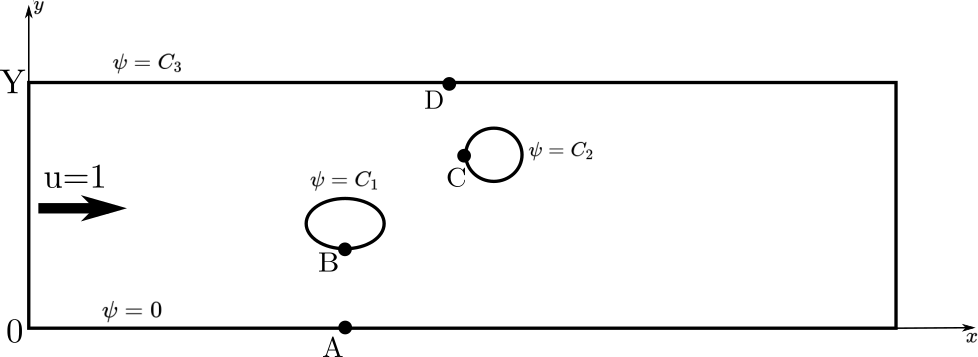
\includegraphics[width=0.8\linewidth]{psi_bc.png}
\caption{Область течения в задаче обтекания}
\label{fig:psi_bc}
\end{figure}

Пусть скорость набегающего потока равна единице на всей входной границе.
На нижней границе положим $\psi_A=0$.
На входной границе получим
\begin{equation}
    \dfr{\psi}{y} = 1 \; \hence \; \psi_{in}(y) = y + \psi_A = y.
\end{equation}
Исходя из значения $\psi_{in}$ на верхней границе можно записать
\begin{equation*}
    \psi_D = \psi_{in}(Y) = Y.
\end{equation*}

Для определения $\psi$ на первом из двух препятствий рассмотрим траекторию $AB$:
\begin{equation*}
    \dfr{\psi}{s} = u_n \; \hence \; \psi_B = \int_A^B u_n ds + \psi_A = Q_{AB},
\end{equation*}
где $s$ - касательная к этой траектории, $n$ -- нормаль к ней, $Q_{AB}$ -- расход
жидкости поперёк траектории $AB$. Вследствии несжимаемости можно
использовать любую из возможных положений точек $A$, $B$ на границах и любую из реализаций траектории.

Аналогично для второго тела можно записать
\begin{equation*}
    \psi_C = Q_{AC} = Q_{AB} + Q_{BC}.
\end{equation*}

\subsection{Задание для самостоятельной работы}

Для расчитанного ранее течения в каверне расчитать скалярные поля функции тока и завихренности.

\begin{itemize}
\item
Сначала для вычисления завихренности использовать формулы
\eqref{eq:omega_approx} для внутренних
и \eqref{eq:omega_approx_bc} для граничных узлов.
\item
Затем полученную завихренность использовать для вычисления $\psi$.
Для этого необходимо собрать и решить систему линейных уравнений, где внутренним узлам
будет соответствовать разностная схема \eqref{eq:psi_slae},
а для граничных -- условие $\psi_{i,j} = 0$. 
\item
Полученные поля сохранить в vtk, добавив
строки
\begin{minted}[linenos=false]{c++}
VtkUtils::add_point_data(psi, "psi", filepath);      // найденный вектор psi
VtkUtils::add_point_data(omega, "omega", filepath);  // найденный вектор omega
\end{minted}
в функцию сохрания на основной сетке 
\begin{minted}[linenos=false]{c++}
void Cavern2DSimpleWorker::save_current_fields(size_t iter){
    if (_writer_all){
        ...
@\end{minted}
\end{itemize}
